\section{Увод - Шта је TLA?}
TLA је језик који за писање и провервање спецификација или дизајнирање система.
Када имамо нашу спецификацију тада га можемо користити за
тестирање грешака у дизајну и пре него што почнемо са самом имплементацијом система.
Развијен је од стране Леслија Лампорта, који је такође осмислио језик \LaTeX
што је скраћеница од Лампортов \TeX.
TLA је скраћеница за Temportal Logic of Actions (Темпорале Логике Акција).

\subsection{Инсталација}

Да бисмо почели да пишемо и проверавамо TLA+ спецификације, потребно је инсталирати следеће алате:

\begin{itemize}
    \item \textbf{Java} -- TLA+ алати захтевају Java Runtime Environment (JRE 8 или новији).
    Може се преузети са \url{https://www.java.com}.

    \item \textbf{TLA+ Toolbox} -- званични IDE за TLA+, доступан на
    \url{https://github.com/tlaplus/tlaplus/releases}.
    Садржи TLC model checker и TLAPS (TLA+ Proof System).

    \item \textbf{VS Code додатак (алтернатива)} -- за кориснике Visual Studio Code,
    постоји додатак \texttt{TLA+ by alygin} доступан у VS Code Marketplace-у.
\end{itemize}

\subsubsection{Кораци инсталације (TLA+ Toolbox)}

\begin{enumerate}
    \item Преузети инсталациони пакет са званичне странице за свој оперативни систем.
    \item Покренути инсталацију и пратити упутства.
    \item Покренути Toolbox и креирати нови пројекат: \textit{File > Open Spec > Add New Spec}.
    \item Написати прву спецификацију и покренути TLC model checker.
\end{enumerate}
\subsubsection{Кораци инсталације (VS Code еditor)}
У овим материјалима користићемо VS Code editor (надље само \textbf{вс едитор})
и објаснићемо примере и инсталацију на примеру њега у оперативном систему линукс. Напомињемо да се TLA+ Toolbox
више не одржава, али да се и даље може скинути и користити. Вс едитор је постао
стандард за писање спецификација и TLA се може користити кроз њега као додатак.
Иначе напомињемо да је вс едитор постао популаран едитор за разне програмске језике
управо због модуларности коју пружа богат избор додатака.

Изаберемо иконицу са додацима где се они инсталирају као на слици 1.
\begin{figure}[H]
    \centering
    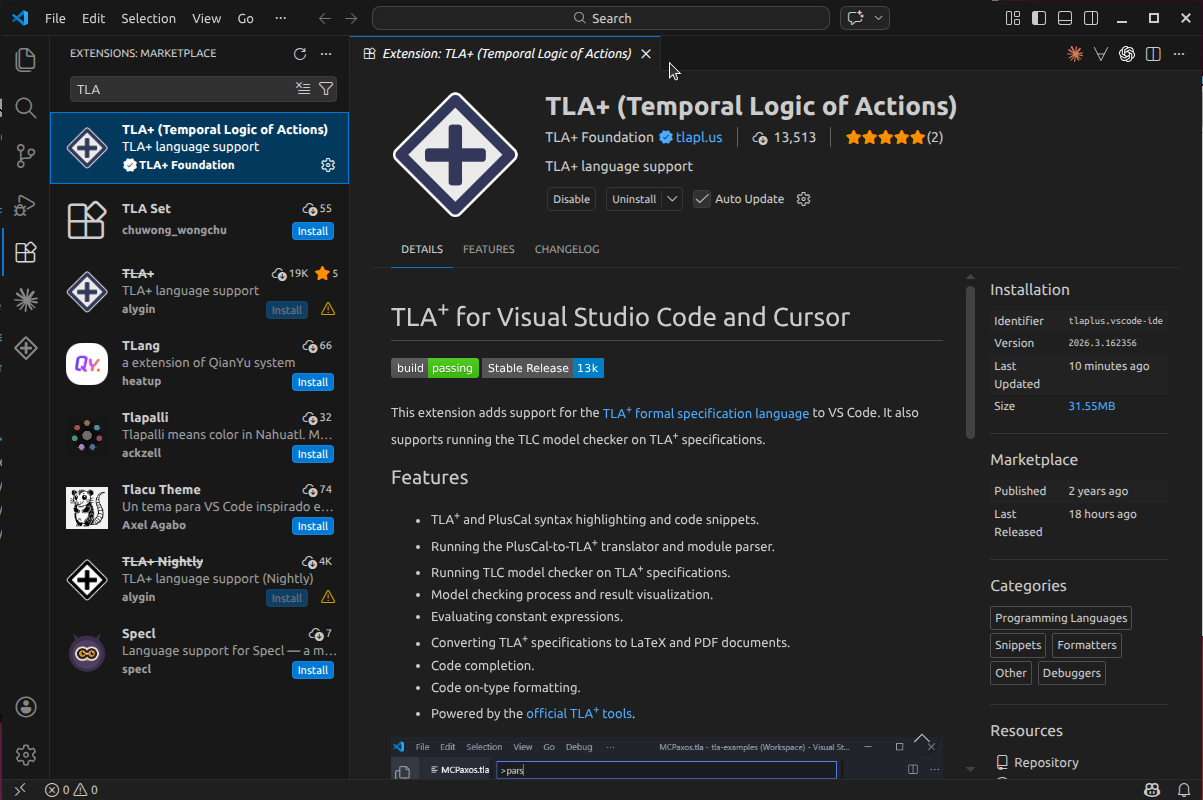
\includegraphics[width=0.7\textwidth]{Images/Instalacija.png}
    \caption{Инсталација TLA+ додатка у VS Code}
\end{figure}
Приликом избора додатка који ћемо инсталирати у претрагу укуцамо
TLA и одаберемо додак као на слици. На крају процеса едитор треба да
изгледа као на слици 2.
\begin{figure}[H]
    \centering
    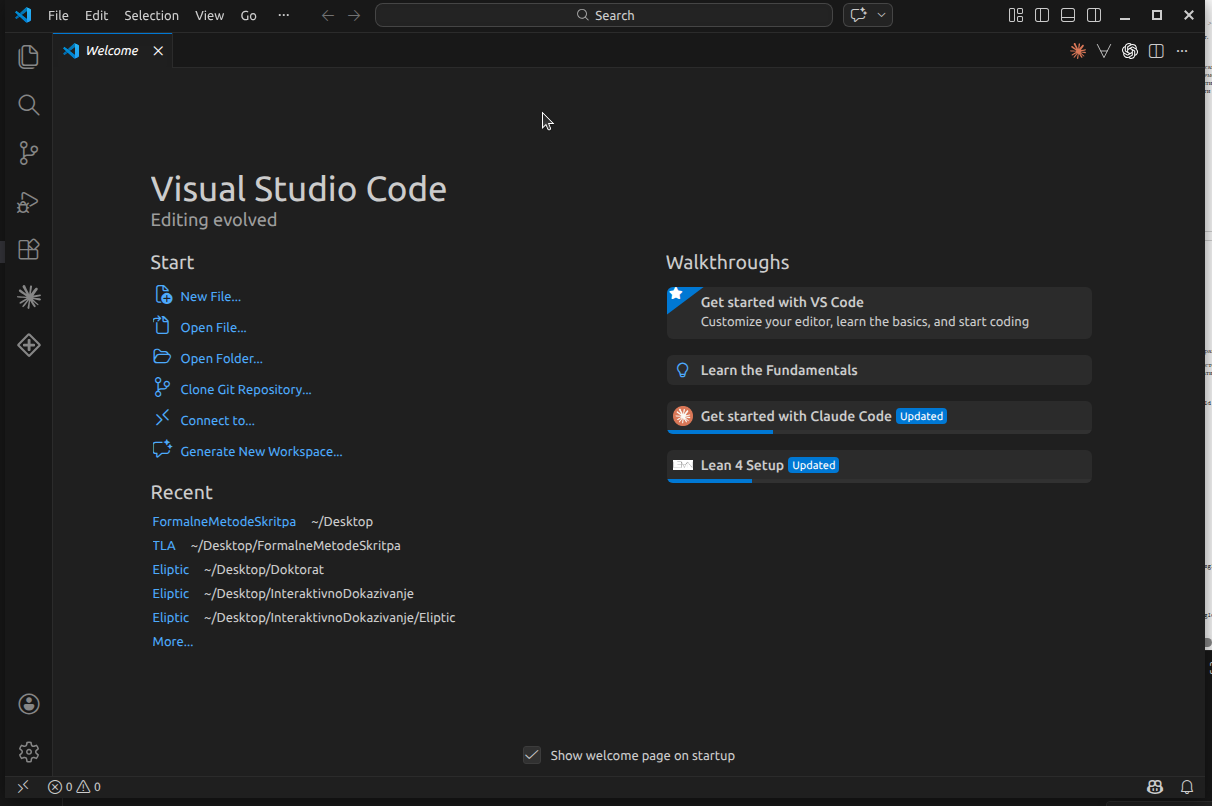
\includegraphics[width=0.7\textwidth]{Images/VSEditor.png}
    \caption{VS Code едитор са TLA+ додатком}
\end{figure}

Сада дајемо мали пример TLA спецификације како би тестирали дали окружење ради добро.

\begin{lstlisting}
---- MODULE Counter ----
EXTENDS Naturals

VARIABLE counter

Init ==
    counter = 1

Next ==
    IF counter < 10
    THEN counter' = counter + 1
    ELSE counter' = counter

Spec ==
    Init /\ [][Next]_counter
====
\end{lstlisting}
У едитору ћемо направити нов текстуални фајл са наставком \textbf{.tla} и
прекопирати претходни код. Пошто смо инсталирали TLA+ додатак на десни клик мишшем
добијамо могућност да одаберемо \textbf{Check model with TLC} као и
 \textbf{Check and debug model with TLC}. \textbf{TLC} је скраћеница за \textbf{TL checker}
и он нам служи да пронађе грешке у нашем дизајну система.
\begin{figure}[H]
    \centering
    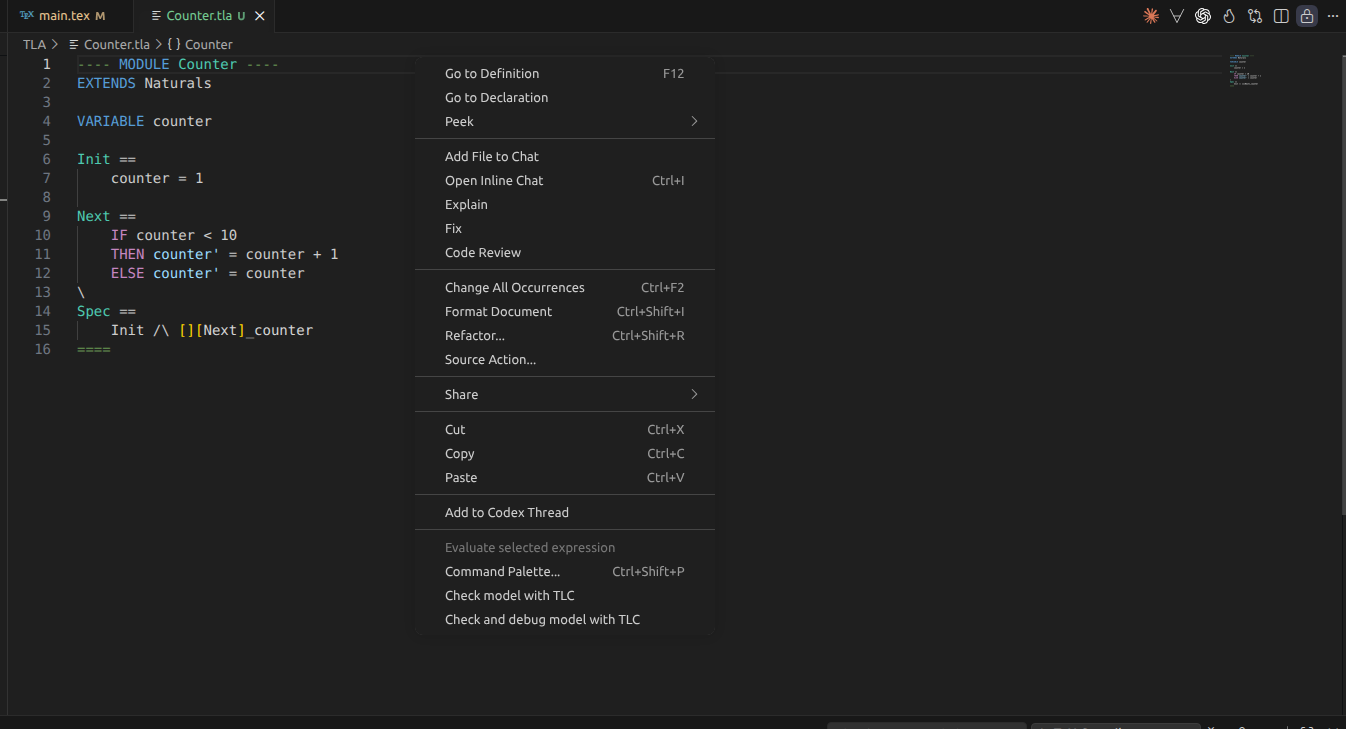
\includegraphics[width=0.7\textwidth]{Images/UvodniPrimer1.png}
    \caption{Код са TLA+ додатком}
\end{figure}
Када кликнемо да проверимо модел тада се може јавити грешака као на следећој слици.
\begin{figure}[H]
    \centering
    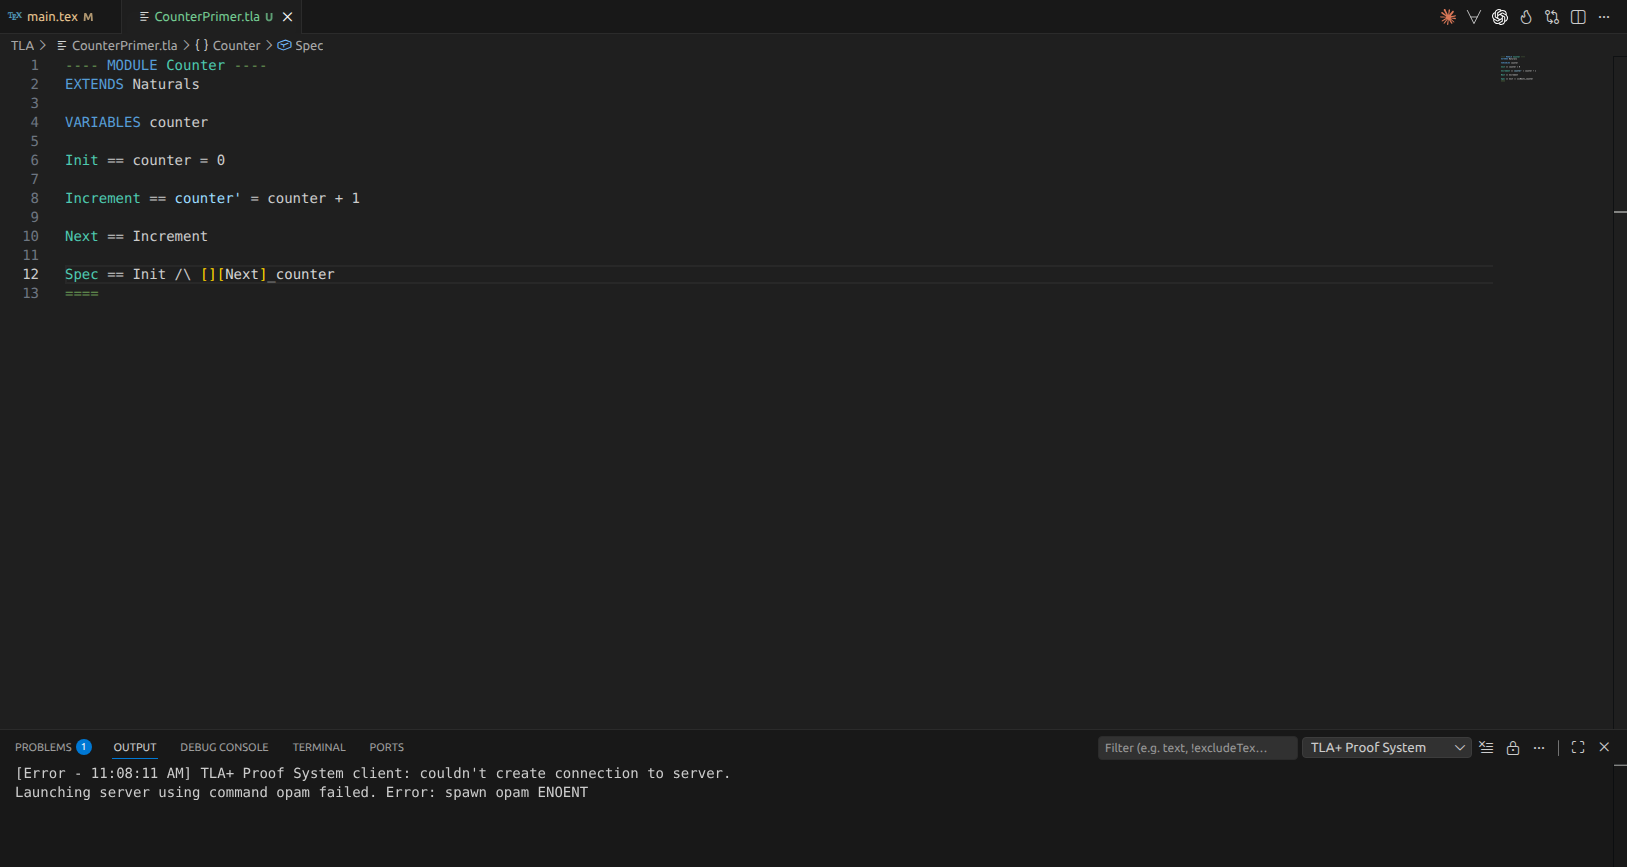
\includegraphics[width=0.7\textwidth]{Images/Greska.png}
    \caption{Грешка при покретању провере}
\end{figure}
Грешка се јавља зато што \textbf{TLAPS - TLA Proof System} покушава да користити
програмски језик \textbf{OCaml}. Ова грешка се на линукс оперативном систему једноставно
решава инсталацијом пакета \textbf{OPAM} следећим командама у терминалу:
\begin{lstlisting}
sudo apt update
sudo apt install opam m4 pkg-config zlib1g-dev gawk time
\end{lstlisting}
Напомињемо да су ово команде за линукс/\textbf{Ubuntu}, ако користите неку другу
дистрибуцију линукса потражите одговарајуће команде.
Уз сваку tla спецификацију (.tla) фајл, такође нам је потребан и конфигурациони
фајл са наставком (.cfg) који нам говори шта су почетна стања, како се прелази у
следеће стање, константе итд.
\begin{lstlisting}
CONSTANTS
    greeting = "Hello"

INIT Init
NEXT Next
\end{lstlisting}
Конфигурациони фајл са претходним кодом морамо да сачувамо у исти фолдер где се налази
и наша спецификација, такође ти фајлови морају имати исто име као и прва линија
у спецификацији (\textbf{Counter.tla}, \textbf{Counter.cfg}).
\begin{lstlisting}
---- MODULE Counter ----
\end{lstlisting}

Кључне ствари које морамо да имамо за сваку спецификацију су:
\begin{enumerate}
    \item Спецификациони фајл са наставком \textbf{.tla}.
    \item Конфигурациони фајл са наставком \textbf{.cfg}.
    \item Они морају да имају исто име, као и име у првој линији у спецификацији.
\end{enumerate}

Пошто смо све урадили, када покренемо проверу спецификације, ако је све у реду
добијамо успех као на слеће две слике.


\begin{figure}[H]
    \centering
    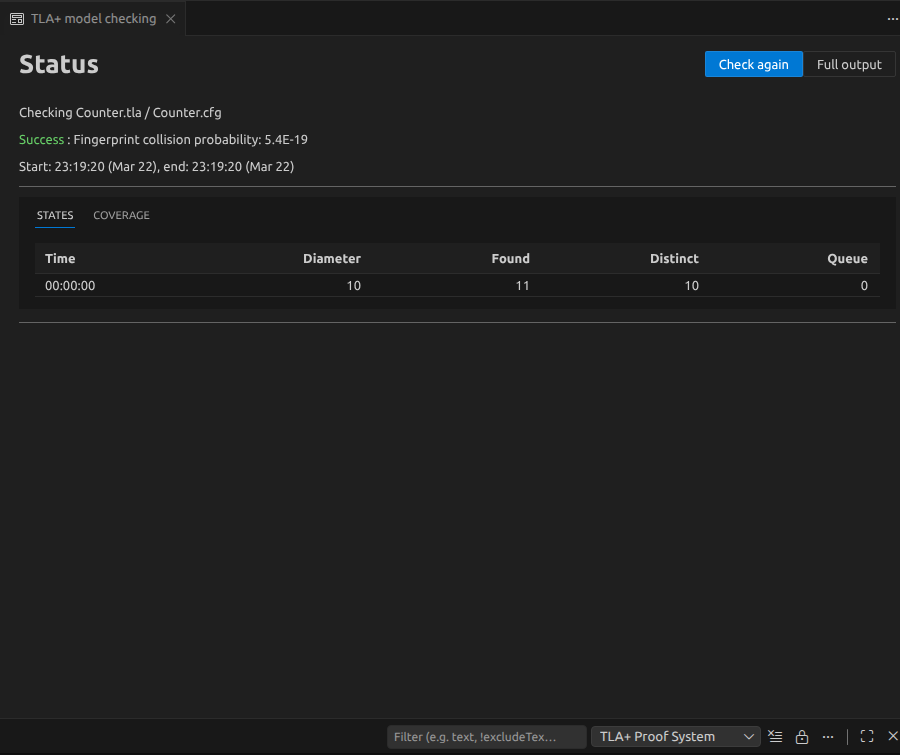
\includegraphics[width=0.7\textwidth]{Images/Uspeh2.png}
    \caption{Успех провера стања}
\end{figure}
\begin{figure}[H]
    \centering
    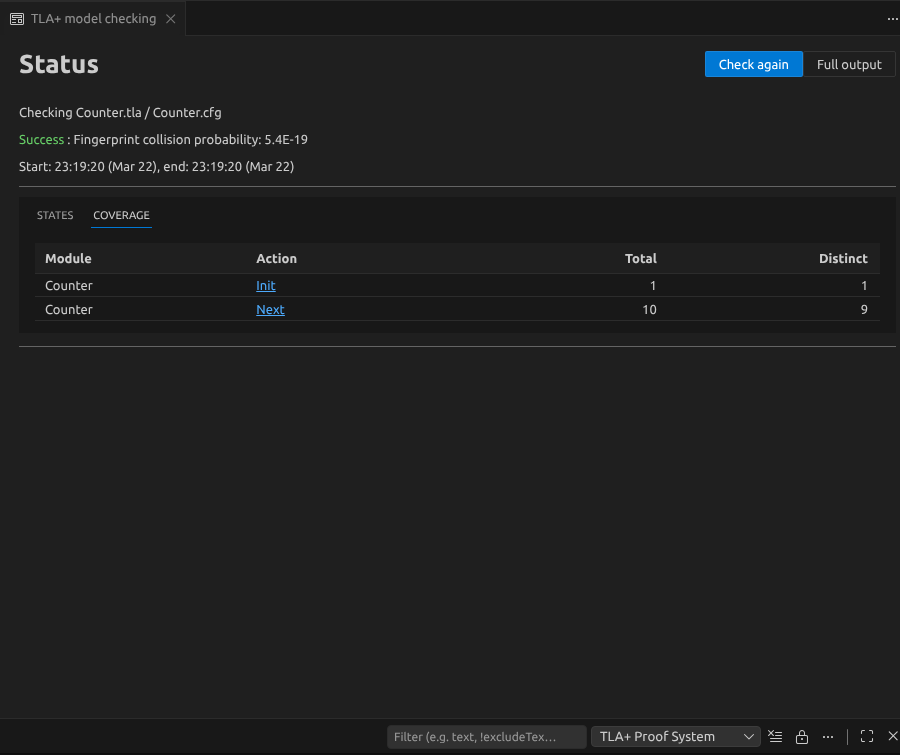
\includegraphics[width=0.7\textwidth]{Images/Uspeh1.png}
    \caption{Успех провера покривености}
\end{figure}
Ово значи да смо успешно успели да инсталирамо tla на линуксу и да наша прва спецификација
система ради без грешке. У следећем поглављу ћемо корак по корак објашњавати шта који део
спецификације значи и чему служи.

\newpage
